\documentclass[9pt]{IEEEtran}

\usepackage[english]{babel}
\usepackage{graphicx}
\usepackage{epstopdf}
\usepackage{fancyhdr}
\usepackage{amsmath}
\usepackage{amsthm}
\usepackage{amssymb}
\usepackage{url}
\usepackage{array}
\usepackage{textcomp}
\usepackage{listings}
\usepackage{hyperref}
\usepackage{xcolor}
\usepackage{colortbl}
\usepackage{float}
\usepackage{gensymb}
\usepackage{longtable}
\usepackage{supertabular}
\usepackage{multicol}
\usepackage{tabu}
\usepackage{verbatim}

\usepackage[utf8x]{inputenc}

\usepackage[T1]{fontenc}
\usepackage{lmodern}
\input{glyphtounicode}
\pdfgentounicode=1


\DeclareGraphicsExtensions{.pdf,.png,.jpg,.eps}

% correct bad hyphenation here
\hyphenation{op-tical net-works semi-conduc-tor trig-gs}

% ============================================================================================

\title{\vspace{0ex}
Data Extractor}

\author{Timotej Kovač\vspace{-4.0ex}}

% ============================================================================================

\begin{document}

\maketitle

\section{Introduction}

TODO

\section{Selection of optional web pages}

For our first website we have chosen a detailed description page of a product available on web store Mimovrste~\ref{mimovrste}.
Here we have chosen some interesting fields that we might be useful as shown in figure ~\ref{fig_mimovrste}.
These were:
\begin{itemize}
\item{tags*, which further describe the item as having a discount, being a recommended product, etc.";}
\item{title;}
\item{description;}
\item{old price*, which states the price before the now discounted price;}
\item{price, which states the current price;}
\item{savings*, which represents the percentage saved;}
\item{availability, which states when the product will be available for shipment.}
\end{itemize}
Fields above marked with an asterisk don't appear always and are therefore optional.

\begin{figure}[ht]
    \centering
    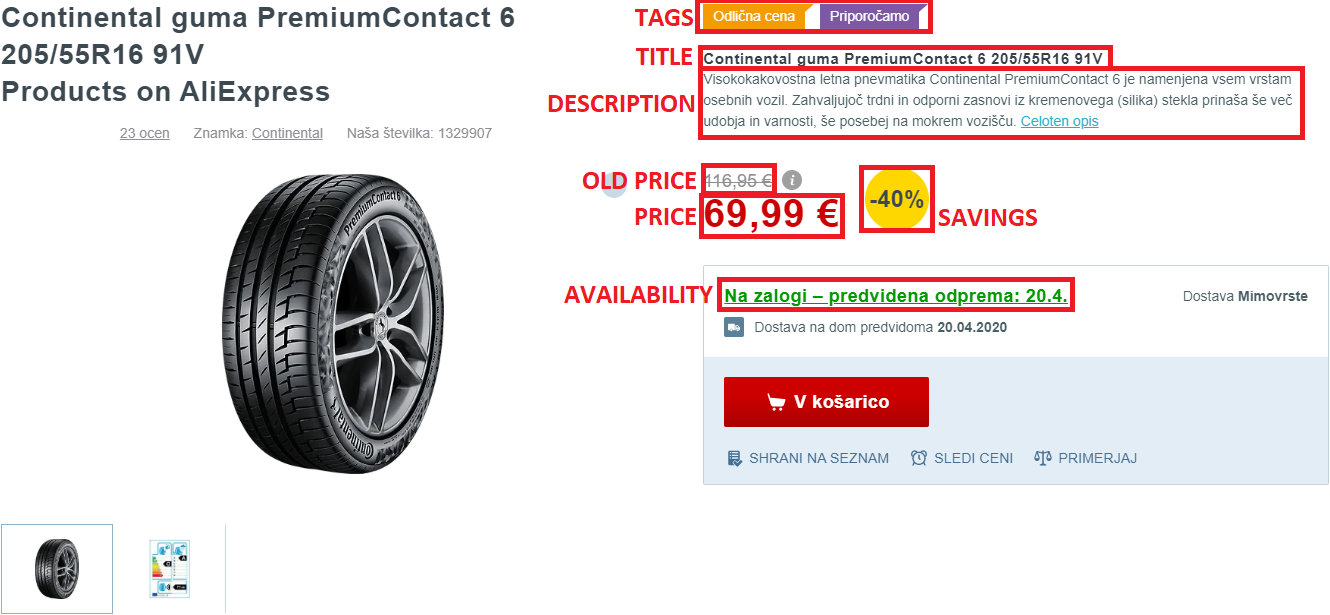
\includegraphics[width=1\columnwidth]{mimovrste.png}
    \caption{Web store mimovrste.si with tagged fields that we used for extraction of web content.}
    \label{fig_mimovrste}
\end{figure}

For our second website we have chosen a page containing multiple items in a grid pattern on a web site Ceneje~\ref{ceneje}.
Here we have chosen the fields listed bellow:
\begin{itemize}
\item{image;}
\item{title;}
\item{min price, which states the minimal price in all of the stores that provide the product;}
\item{number of stores, which states the number of stores that provide the product;}
\item{action, which states what the button does either takes the user to a particular web store or to a list of webstores still on the same ceneje.si domain.}
\end{itemize}
Here none of the fields are optional but some do vary as they may contain some other words in front of the fields or are ads which have a slightly different structure.
This too can be seen in figure~\ref{fig_ceneje}.

\begin{figure}[ht]
    \centering
    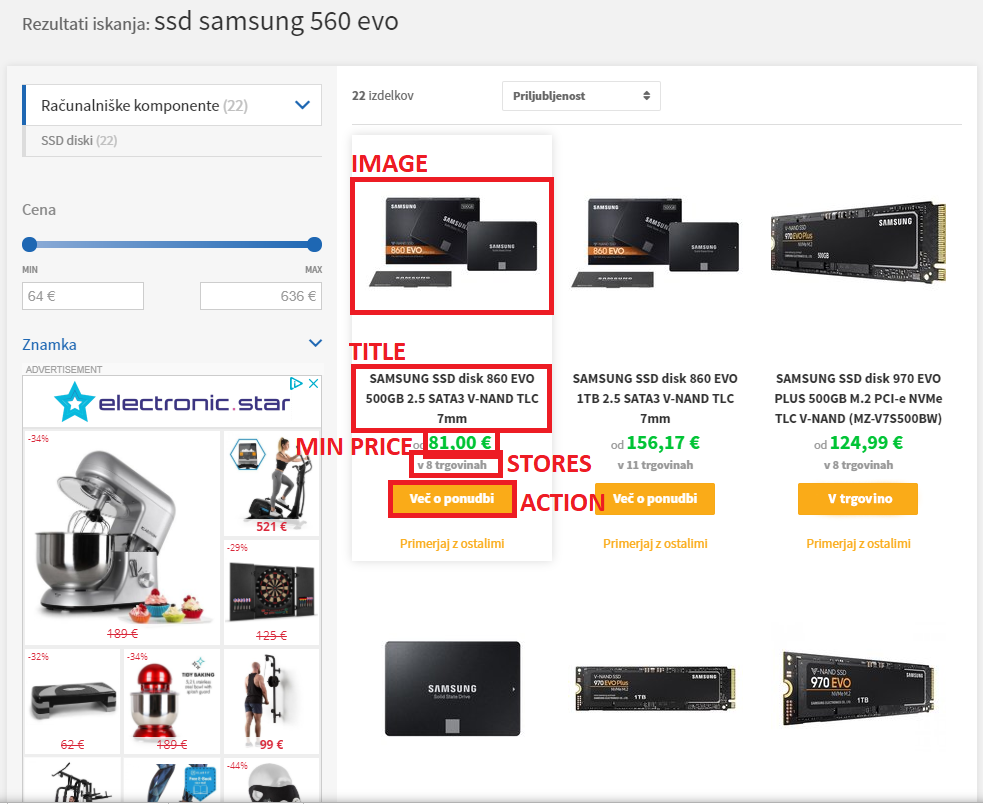
\includegraphics[width=1\columnwidth]{ceneje.png}
    \caption{Web site ceneje.si with tagged fields that we used for extraction of web content.}
    \label{fig_ceneje}
\end{figure}

\section{Regular Expressions Implementation}

rtvslo.si
\begin{itemize}
\item{title: <h1>(.*?)</h1>}
\item{}
\item{}
\item{}
\item{}
\end{itemize}

\section{XPath Implementation}

TODO

\section{Automatic Web Extraction Implementation}

TODO 

\section{Conclusion}

~\cite{jauntium, robots_txt, postgres}
TODO

\bibliographystyle{IEEEtran}
\bibliography{main}

\end{document}
